\documentclass{article}
\usepackage{amsmath}
\usepackage{graphicx}
\usepackage{float}
\usepackage{hyperref}
\usepackage{fancyvrb}
\usepackage{enumitem}
\usepackage{matlab-prettifier}
\usepackage{tcolorbox}  % For rounded boxes
\usepackage{listings}
\setlength{\parindent}{0pt}
\graphicspath{{../images/}}

\lstset{
    basicstyle=\ttfamily\footnotesize,  % Custom font style and size
    keywordstyle=\color{blue}\bfseries, % Custom keyword style
    commentstyle=\color{gray},          % Custom comment style
    morekeywords={unsigned, char, int, void}, % Specify keywords
    backgroundcolor=\color{gray!10},    % Light gray background for code
    columns=fullflexible,
    keepspaces=true,
    breaklines=true,
    language=C++,                      % Specify the language
    style=Matlab-Pyglike,
    escapeinside={(@}{@)}
}

% Rounded box style
\tcbset{
    colframe=black!75!white,    % Border color
    colback=gray!10,            % Background color
    boxrule=0.5pt,              % Border thickness
    arc=6pt,                    % Rounded corners
    outer arc=6pt,
    top=5pt,                    % Padding
    bottom=5pt,
    left=5pt,
    right=5pt,
    fonttitle=\bfseries,        % Bold title font
}


\title{CS663: Digital Image Processing - Homework 4}
\author{Harsh $\vert$ Pranav $\vert$ Swayam} 
\date{October 22, 2024}

\begin{document}

\maketitle
\section{Homework 4 - Question 5}

Our classifier is unaware of the concept of a person not being present in the training set. This is a problem because the classifier will always try to find the closest match, even if the person is not present in the training set. This will lead to them being incorrectly identified as the closest matching person in the training set.
\vspace{5pt}

To analyze a suitable method for identifying people as not being present in the original training set, we considered a few ideas. Most of them revolved around the idea of considering a threshold for some form of error, be that the recognition error or the distance between the test image and the closest image in the training set, or with all images with the same index as the closest image, or even just all images in the training set. 
\vspace{5pt}

In the end, we took the simplest approach of considering the error with the closest image, and if that error was above a certain threshold, we would consider the person as not being present in the training set.

Plotting the recognition rate and mean recognition error for images, we see that the recognition rate is quite high starting from \texttt{k} values as low as 10, and remain mostly stable. 

\begin{figure}[!htb]
    \centering
    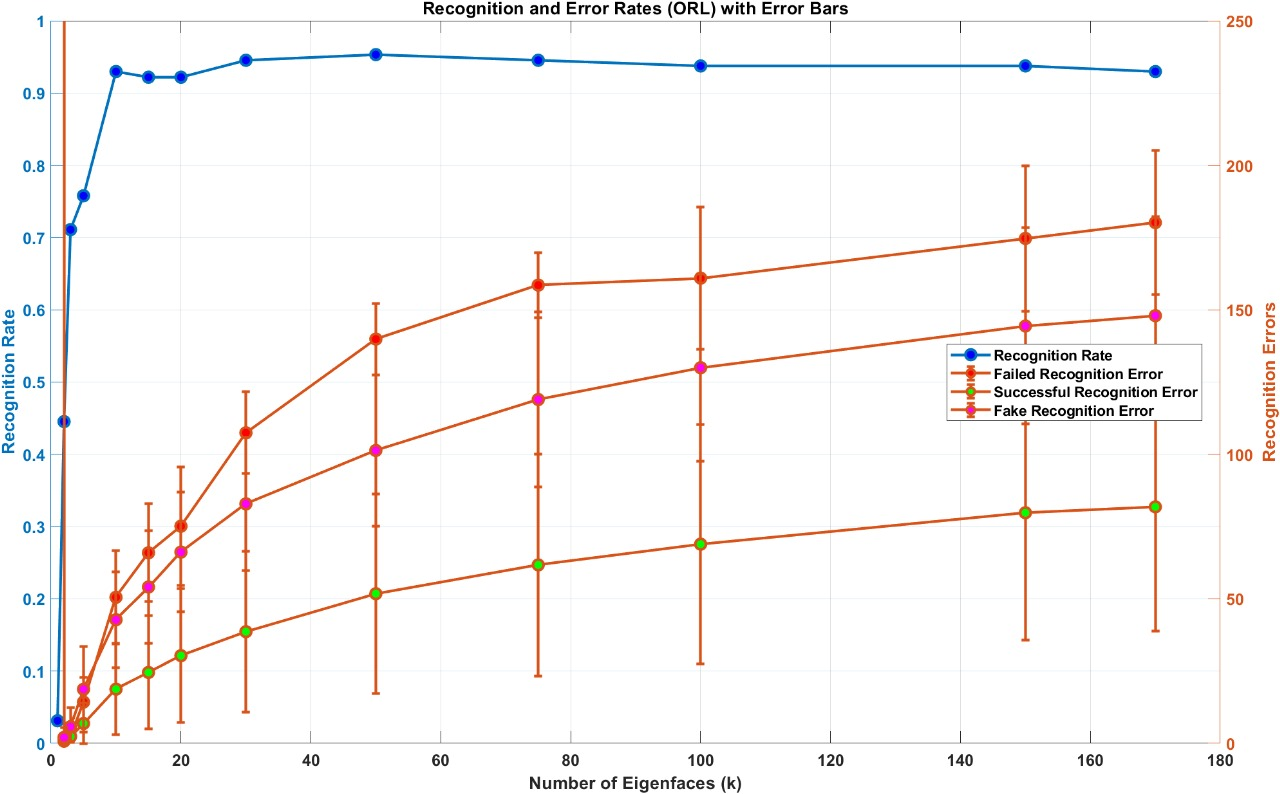
\includegraphics[width=0.65\textwidth]{simple_plot.jpg}
    \caption{Recognition Rate and Errors for different classes (ORL dataset)}
\end{figure}
\begin{figure}[!htb]
    \centering
    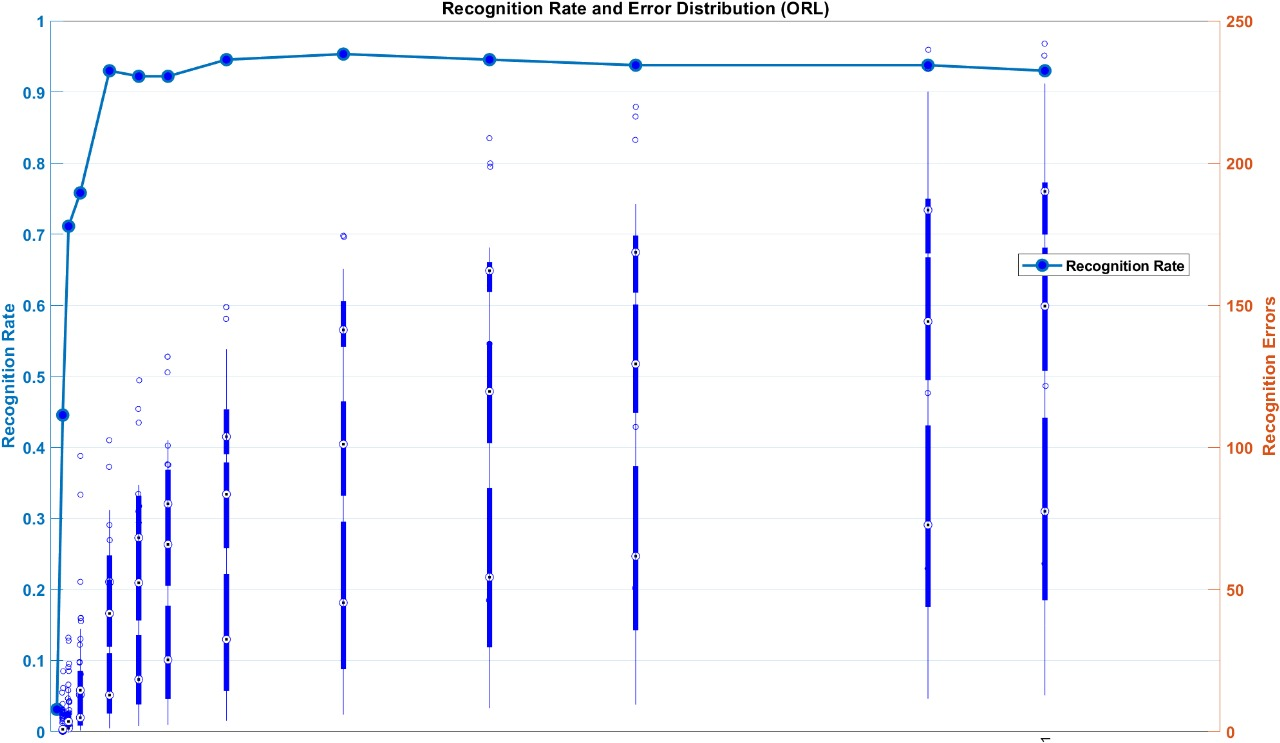
\includegraphics[width=0.65\textwidth]{box_plot.jpg}
    \caption{Recognition Rate and Errors box-whiskers for different classes}
\end{figure}
% \newpage

While correctly labelled images and images with no actual matching identity have sufficient separation, the images with incorrect labels lie between the two. 

From the graph, we see that the separation between distributions relative to their length is the highest for \texttt{k} $= 50$. This should allow for the least overlap between ranges. 
\\
We shall now vary the threshold value to maximize select evaluation metrics. We shall consider the F1 score, accuracy, and recall.

\newpage
First, we define positive cases as images identified as not being in the training set, and negative cases as images identified as being in the training set.
\begin{tcolorbox}[title={Normal Confusion Matrix}]
    \begin{lstlisting}
        Best Threshold: 67, Best F1 Score: 0.609524
        Best Specificity: 0.679688
        Best Accuracy: 0.743750
        Best Recall: 1.000000
        Best Confusion matrix:
        TP: 32  FP: 41
        FN: 0   TN: 87

        ------------------------------
        Best Threshold: 152, Best Accuracy: 0.812500
        Best Specificity: 1.000000
        Best F1 Score: 0.117647
        Best Recall: 0.062500
        Best Confusion matrix:
        TP: 2   FP: 0
        FN: 30  TN: 128

        ------------------------------
        Best Threshold: 50, Best Recall: 1.000000
        Best Specificity: 0.546875
        Best F1 Score: 0.524590
        Best Accuracy: 0.637500
        Best Confusion matrix:
        TP: 32  FP: 58
        FN: 0   TN: 70
    \end{lstlisting}
\end{tcolorbox}
\newpage
Next, we consider the confusion matrix excluding images of people in the training set with incorrect labels, to see if the results are any different.
\begin{tcolorbox}[title={Confusion Matrix (excluding images with incorrect labels)}]
    \begin{lstlisting}
        Best Threshold: 67, Best F1 Score: 0.646465
        Best Specificity: 0.713115
        Best Accuracy: 0.772727
        Best Recall: 1.000000
        Best Confusion matrix:
        TP: 32  FP: 35
        FN: 0   TN: 87

        ------------------------------
        Best Threshold: 110, Best Accuracy: 0.831169
        Best Specificity: 0.950820
        Best F1 Score: 0.480000
        Best Recall: 0.375000
        Best Confusion matrix:
        TP: 12  FP: 6
        FN: 20  TN: 116

        ------------------------------
        Best Threshold: 50, Best Recall: 1.000000
        Best Specificity: 0.573770
        Best F1 Score: 0.551724
        Best Accuracy: 0.662338
        Best Confusion matrix:
        TP: 32  FP: 52
        FN: 0   TN: 70
    \end{lstlisting}
\end{tcolorbox}

We can see that while accuracy is biased towards increasing TN with the highest possible count, and the recall is biased towards the making FN 0 by reducing the threshold drastically, F1 scores seems to be the most balanced metric. However, the threshold given by best accuracy gives more TPs on the exclusion of images with incorrect labels.
\vspace{5pt}

In the end, the choice of threshold should depend on the application.
\end{document}